
\section{Experiment Result}

In this paragragh we will try to explain how we're going to evaluate our work. We plan to evalute our reinforcement learning model in different aspects, including converge rate, suceess rate and reaction time.

Because the model is designed for a preset sector with specific routes and aircraft and the model could be reused in later operations, the time of training is not the most important thing we consider, but we still hope that the algorithm could converge as soon as possible. As is mentioned above, the air traffic control process is fatal and latency-sensitive, so the success rate and the reaction time are both worth careful consideration.

We propose to record the number of aircraft that leave the sector without collision in the training process and the test process, while the time that agents take each reaction will only be recorded in the test process to ensure that the model is fixed and unchanged.

With such data, we could draw the line chart to show how the success rate raise during the trainging process, and the box-plot to show how our model perform during the test process. The mean and median of the interpretation time could be calculated to show how fast the model react once it's asked to give decision advisories.

\begin{figure}[!htbp]
    \centering
    \subfigure[\label{fig:10aircraft}Episodes vs. Pass Through]{
        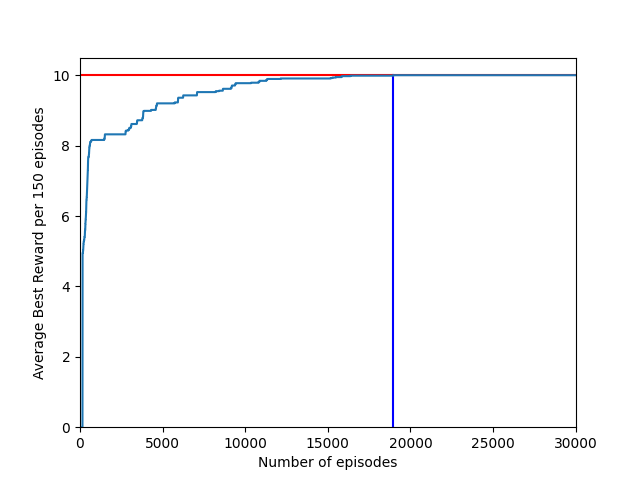
\includegraphics[width=0.3\columnwidth]{images/10aircraft.png}
    }
    \subfigure[\label{fig:30vs50}Influence of Aircrafts]{
        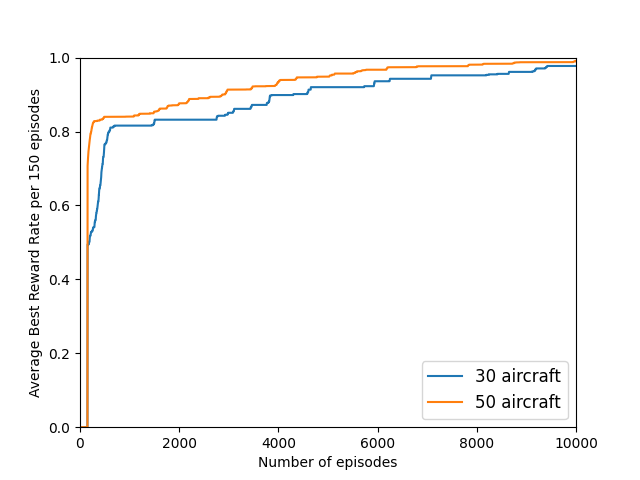
\includegraphics[width=0.3\columnwidth]{images/30vs50.png}
    }
    \subfigure[\label{fig:intruders}Influence of Intruders]{
        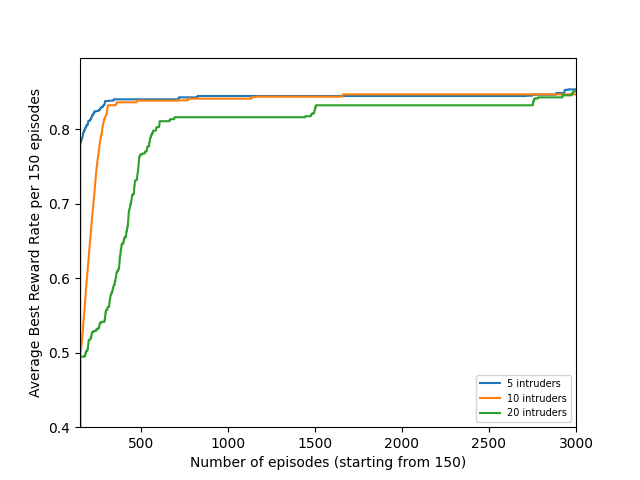
\includegraphics[width=0.3\columnwidth]{images/intruder_influence.png}
    }
    \caption{Experimental Results}
    \label{fig:exp_result}
\end{figure}

From Figure \ref{fig:10aircraft} we can see that the model is actually trainable under our settings. Note that we didn't plot the reward we get every episode since it can vibrates a lot and will cause trouble for us to see the trend. Also the smallest diffence between the reward each time is 2 rather than 1 since we defined the reward as the number of aircraft that leave the sector successfully. Instead, we record the average reward every 150 episodes.

We also try to check whether using information from some of rather than all of other planes could be effective. We fix the n-sate as 5, so the sample rate could change from 50\% to 16.7\% when we change the maximum number of aircrafts in the sector from 30 to 50. From Figure \ref{fig:30vs50} we can see that the convergence result didn't get worse.

The number of intruders could also influence the converge speed. Checking the \textit{150-th} to the \textit{3000-th} episodes, we can see such result. The reason might be more intruders potentially increase the difficulty to pass through. However, this will not influence the process of convergence. The result is shown on Figure \ref{fig:intruders}.